\chapter{Memory management}
In 32-bit operating systems, pointers are 4-byte objects, i.e.,\@ have a private 4~GB virtual address space, half available to a process. Win64 provides 64-bit pointers, enlarging virtual address space.

Programs can create independent memory ``heaps'' and can map files to memory.

\begin{figure}[hbtp]
\centering
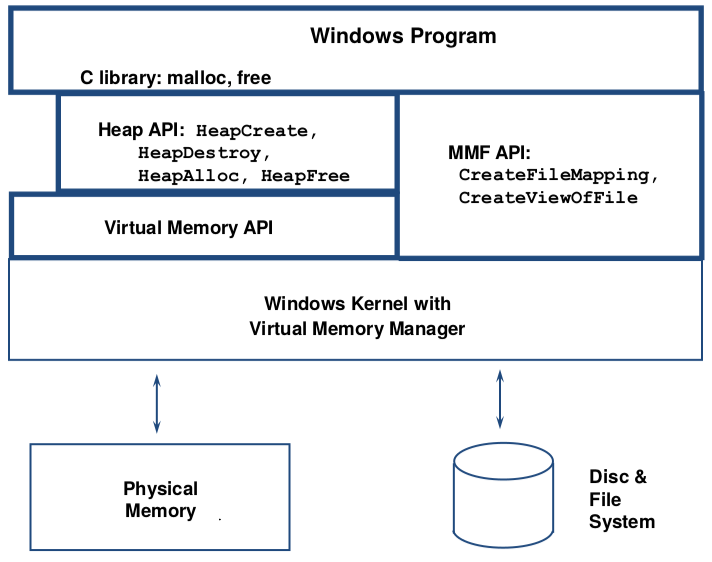
\includegraphics[scale=0.35]{images/windows_memory_management/architecture.png}
\caption{Architecture}
\end{figure}

\section{Memory management and heaps}
A \emph{heap} is a pool of memory within a process virtual address space. Commonly, every process has a default process heap. In Windows, a process may have more than on heap, providing some benefits:
\begin{itemize}
\item Fairness between threads and between users, i.e.,\@ having their own heaps, they do not ``steal'' space each others;
\item Allocation efficiency, i.e.,\@ fixed size blocks in each heap;
\item Deallocation efficiency, i.e.,\@ deallocation of a complete data structure is possible in one single call;
\item Locality of reference efficiency, i.e.,\@ in smaller heaps, it is easier to exploit locality principle because data are ``closer''.
\end{itemize}

Every heap has a handle. The programmer can use the process heap or create new ones. \texttt{HANDLE GetProcessHeap()} returns the handle for the process' heap or \texttt{NULL} on failure.

Multiple heaps may limit fragmentation by allocating similar data in the same heap. In every dynamic allocation scheme, sooner or later the allocation pattern will be an alternation of small free blocks and allocated frames. Exploiting multiple heaps, it is possible to reduce this type of fragmentation.

\subsection{Heap management}
\begin{verbatim}
HANDLE HeapCreate (
  DWORD flOptions,
  DWORD dwInitialSize,
  DWORD dwMaximumSize
);
\end{verbatim}

\paragraph{Returned value}
\begin{itemize}
\item A heap handle on success;
\item \texttt{NULL} on failure.
\end{itemize}

\paragraph{Parameters}
\begin{description}
\item [\texttt{flOptions}] Combination of two flags:
\begin{description}
\item [\texttt{HEAP\_GENERATE\_EXCEPTIONS}] By generating exceptions, it is possible to avoid explicit testing after each heap management call;
\item [\texttt{HEAP\_NO\_SERIALIZE}]
\end{description}
\item [\texttt{dwInitialSize}]
\item [\texttt{dwMaximumSize}] Maximum heap size:
\begin{description}
\item [\texttt{0}] ``Growable heap'' without any fixed limit;
\item [non-zero] ``Non-growable heap''. The entire block is allocated from the virtual address space but only the initial size is committed in the paging file.
\end{description}
\end{description}

\begin{verbatim}
BOOL HeapDestroy (HANDLE hHeap);
\end{verbatim}
Do not destroy the process' heap, obtainable using \texttt{GetProcessHeap()}. By using \texttt{HeapDestroy}, mo data structure traversal code is necessary and it is not needed to deallocate each individual data structure element, which be time-consuming.

\paragraph{Returned value}
\begin{itemize}
\item \texttt{TRUE} on success;
\item \texttt{FALSE} on failure.
\end{itemize}

\paragraph{Parameter}
\begin{description}
\item [\texttt{hHeap}] Heap handle generated using \texttt{HeapCreate}.
\end{description}

\begin{verbatim}
LPVOID HeapAlloc (
  HANDLE hHeap,
  DWORD dwFlags,
  DWORD dwBytes
);
\end{verbatim}

\paragraph{Returned value}
\begin{itemize}
\item A pointer to the allocated memory block;
\item \texttt{NULL} on failure, unless exception generation is specified.
\end{itemize}

\paragraph{Parameters}
\begin{description}
\item [\texttt{hHeap}] Heap generated using \texttt{HeapCreate} or obtained with \texttt{GetProcessHeap}.
\item [\texttt{dwFlags}] Combination of:
\begin{description}
\item [\texttt{GENERATE\_EXCEPTIONS}]
\item [\texttt{NO\-SERIALIZE}]
\item [\texttt{HEAP\_ZERO\_MEMORY}]
\end{description}
\item [\texttt{dwBytes}] Number of bytes to allocate.
\end{description}

\begin{verbatim}
BOOL HeapFree (
  HANDLE hHeap,
  DWORD dwFlags,
  LPVOID lpMem
);
\end{verbatim}

\paragraph{Returned value}
\begin{itemize}
\item \texttt{TRUE} on success;
\item \texttt{FALSE} on failure.
\end{itemize}

\paragraph{Parameters}
\begin{description}
\item [\texttt{hHeap}] It should be the heap that \texttt{lpMem} was allocated from.
\item [\texttt{dwFlags}] It should be zero on \texttt{HEAP\_NO\_SERIALIZE}.
\item [\texttt{lpMem}] It should have a value returned by \texttt{HeapAlloc} or \texttt{HeapReAlloc}.
\end{description}

\begin{verbatim}
LPVOID HeapReAlloc (
  HANDLE hHeap,
  DWORD dwFlags,
  LPVOID lpMem,
  DWORD dwBytes
);
\end{verbatim}

\paragraph{Returned value}
\begin{itemize}
\item A pointer to the reallocated memory block;
\item \texttt{NULL} on failure, unless exception generation is specified.
\end{itemize}

\paragraph{Parameters}
\begin{description}
\item [\texttt{hHeap}] Heap generated using \texttt{HeapCreate} or obtained with \texttt{GetProcessHeap}.
\item [\texttt{dwFlags}] Some essential control blocks:
\begin{description}
\item [\texttt{HEAP\_GENERATE\_EXCEPTIONS} or \texttt{HEAP\_NO\_SERIALIZE}]
\item [\texttt{HEAP\_ZERO\_MEMORY}] Only newly allocated memory is initialized.
\item [\texttt{HEAP\_REALLOC\_IN\_PLACE\_ONLY}] Do not move the block.
\end{description}
\item [\texttt{lpMem}] Existing block in \texttt{hHeap} to be reallocated.
\item [\texttt{dwBytes}] New block size.
\end{description}

\begin{verbatim}
LPVOID HeapSize (
  HANDLE hHeap,
  DWORD dwFlags,
  LPVOID lpMem
);
\end{verbatim}

\paragraph{Returned value}
\begin{itemize}
\item The size of the block;
\item \texttt{0} on failure.
\end{itemize}

\subsection{Heap flags}
\begin{description}
\item [\texttt{HEAP\_NO\_SERIALIZE}] Performance gain, about 15\% in tests, as functions do not provide mutual exclusion to threads accessing the heap. It can safely be used, carefully, if:
\begin{itemize}
\item The process uses only a single thread;
\item Each thread has its own heap(s) that no other thread can access;
\item Mutual exclusion is provided by the programmer to prevent concurrent access to a heap by several threads;
\item \texttt{HeapLock} and \texttt{HeapUnlock} are used.
\end{itemize}
\item [\texttt{HEAP\_GENERATE\_EXCEPTIONS}] Allows to avoid error tests after each allocation.
\end{description}

\section{Memory mapped files}
Mapping virtual memory space directly to normal files rather than the paging file leads to some advantages:
\begin{itemize}
\item No need to perform direct file I/O;
\item Created data structure are save in the file;
\item Possibility to use in-memory algorithm to process data even though the file may be much larger than available physical memory;
\item No need to manage buffers and file data they contain;
\item Multiple process can share memory and the file views will be coherent;
\item No need to consume space in the paging file.
\end{itemize}

\begin{verbatim}
HANDLE CreateFileMapping (
  HANDLE hFile,
  LPSECURITY_ATTRIBUTES lpsa,
  DWORD dwProtect,
  DWORD dwMaximumSizeHigh,
  DWORD dwMaximumSizeLow,
  LPCTSTR lpMapName
);
\end{verbatim}

\paragraph{Returned value}
\begin{itemize}
\item A file mapping \texttt{HANDLE};
\item \texttt{NULL} on failure.
\end{itemize}

\paragraph{Parameters}
\begin{description}
\item [\texttt{hHeap}] Open file handle with protection flags compatible with \texttt{dwProtect}.
\item [\texttt{lpsa}] Usually \texttt{NULL}.
\item [\texttt{dwProtect}] Access mode to the mapped file:
\begin{description}
\item [\texttt{PAGE\_READONLY}] Pages in the mapped region are read only.
\item [\texttt{PAGE\_READWRITE}] Full access if \texttt{hFile} has both \texttt{GENERIC\_READ} access and \texttt{GENERIC\_WRITE} access.
\item [\texttt{PAGE\_WRITECOPY}] When a change occurs in mapped memory, a copy is written to the paging file.
\end{description}
\item [\texttt{dwMaximumSizeHigh}] Low-order 32 bits of the size of the mapping object; \texttt{0} for current file size.
\item [\texttt{dwMaximumSizeLow}] High-order 32 bits of the size of the mapping object; \texttt{0} for current file size. The file is extended if the current file size is small than the map size.
\item [\texttt{lpMapName}] Names the mapping object, allowing other processes to share the object.
\end{description}

\begin{verbatim}
HANDLE OpenFileMapping (
  DWORD dwDesiredAccess,
  BOOL bInheritHandle,
  LPCTSTR lpNameP
);
\end{verbatim}

\paragraph{Returned value}
\begin{itemize}
\item A file mapping \texttt{HANDLE};
\item \texttt{NULL} on failure.
\end{itemize}

\begin{description}
\item [\texttt{dwDesiredAccess}] The access to the file mapping object.
\item [\texttt{bInheritHandle}] If \texttt{TRUE}, a process can inherit the handle. Otherwise, the handle cannot be inherited.
\item [\texttt{lpNameP}] The name of the file mapping object to be opened.
\end{description}

\subsection{Mapping process address space}
\begin{verbatim}
LPVOID MapViewOfFile (
  HANDLE hMapObject,
  DWORD dwAccess,
  DWORD dwOffsetHigh,
  DWORD dwOffsetLow,
  DWORD cbMap
)
\end{verbatim}

\paragraph{Returned value}
\begin{itemize}
\item The starting address of the block, i.e.,\@ file view;
\item \texttt{NULL} on failure.
\end{itemize}

\paragraph{Parameters}
\begin{description}
\item [\texttt{hMapObject}] File-mapping object.
\item [\texttt{dwAccess}] Must be compatible with mapping object's access.
\begin{description}
\item [\texttt{FILE\_MAP\_WRITE}]
\item [\texttt{FILE\_MAP\_READ}]
\item [\texttt{FILE\_MAP\_ALL\_ACCESS}]
\end{description}
\item [\texttt{dwOffsetHigh}] Low-order 32 bits of the offset of the mapped file region.
\item [\texttt{dwOffsetLow}] High-order 32 bits of the offset of the mapped file region.
\item [\texttt{cbMap}] Size in bytes of the mapped region. Zero indicates entire file.
\end{description}
\texttt{dwOffsetHigh} and \texttt{dwOffsetLow} must be a multiple of 64~K. Zero offset means mapping from the beginning of the file.

\texttt{MapViewOfFileEx} is similar, but it is possible to specify an existing address.

\begin{verbatim}
BOOL UnmapViewOfFile (LPVOID lpBaseAddress);
\end{verbatim}
It permits to release file views.

\subsubsection{File mapping limitations}
\begin{itemize}
\item Disparity between Windows' 64-bit file system and 32-bit addressing;
\item A large file, i.e.,\@ greater than 4~GB, cannot be mapped entirely into virtual memory space;
\item Process data space is limited to 2~GB, not usable entirely because only smaller contiguous block are available;
\item Dealing with large files, it is necessary to write code that carefully maps and unmaps file regions as needed.
\end{itemize}

\paragraph{Based pointers}
Pointers used in a mapped file region should be of type \texttt{\_\_based}, i.e.,\@ final address will be composed by a relative part (base) and a relative part.

A conventional pointer refers to the virtual address. This address base will almost certainly be different the next time that file is mapped or a new view is created of the same region, therefore pointer should be \emph{based} on the view address.

\section{Dynamic link libraries}
Building one or more libraries as \emph{static libraries} permits to link these libraries with each project as needed.

This approach simplifies and expedites project building but brings to disk and memory space issues and complicates maintenance which requires relinking and redistribution. Therefore, different programs may use different library versions and cannot use alternate utility implementations for different situations.

\subsection{Dynamic link libraries}
\emph{Dynamic link libraries} solve these and other problems very neatly. Library functions can be linked at load time, i.e.,\@ implicit linking, or at run time, i.e.,\@ explicit linking. In this way, program image can be much smaller, since it does not include library functions.

Multiple programs can share a single DLL. In this way, only a single copy will be loaded into memory, all programs map their process address space to DLL code and each thread will have its own copy of non-shared storage on the stack.

New versions or alternate implementations can be easily developed supplying a new version of the DLL. All programs can use the new version without modification. Exploiting \emph{explicit linking}:
\begin{itemize}
\item Program decides at run time which library version to use;
\item Different libraries may be alternate implementations of the same function;
\item May carry out totally different tasks;
\item The library will run in the same process and threads as the calling process.
\end{itemize}
Multiple Windows processes can share DLL code. Code, when called, runs as part of the calling process and thread, i.e.,\@ library can use the calling process' resources and uses the calling thread's stack. Hence, DLLs must be thread-safe and can also export variables as well as function entry points.

\subsubsection{Implicit linking}
\emph{Implicit linking}, or load time linking, is the easiest of the two techniques.

The executable using the DLL links to an import library (.lib file) provided by the maker of the DLL and always present in the system. The operating system loads the DLL when the executable using it is loaded. The client executable calls the DLL’s exported functions just as if the functions were contained within the executable. This call is split into two parts:
\begin{itemize}
\item First, the linker links the function call to a dummy function ``stub''. Inside the executable there is a table with all the stubs of all DLL’s requested functions.
\item When the executable is loaded, the operating system maps all the stubs with the correct
entry points of the functions in the DLL.
\end{itemize}

\paragraph{Exporting and importing interfaces}
DLL entry point must be declared using the \texttt{\_declspec (dllexport)} storage modifier. Calling program declares the function is to be imported using the \texttt{\_declspec (dllimport)} storage modifier.

Standard technique in include file is to use a preprocessor variable, such as \texttt{MYPROJECT\_EXPORTS}.
\begin{verbatim}
#ifdef MYPROJECT_EXPORTS
#define LIBSPEC _declspec (dllexport)
#else
#define LIBSPEC _declspec (dllimport)
#endif
LIBSPEC DWORD MyFunction (...);
\end{verbatim}
The DLL project defines \texttt{MYPROJECT\_EXPORTS}, while calling application leaves \texttt{MYPROJECT\_EXPORTS} undefined.

It is possible to export and import variables as well as function entry points. 

\subsubsection{Explicit linking}
In \emph{explicit linking}, or run time dynamic linking, the executable using the DLL must make function calls to explicitly load and unload the DLL and to access the DLL’s exported functions. A module uses the \texttt{LoadLibrary()} or \texttt{LoadLibraryEx()} function to load the DLL at run time. After the DLL is loaded, the module calls the \texttt{GetProcAddress()} function to get the addresses of the entry point(s) of the DLL functions. The module calls the exported DLL functions using the function pointers returned by \texttt{GetProcAddress()}: this eliminates the need for an import library. Finally, it free the library calling the \texttt{FreeLibrary()} function.

\begin{verbatim}
HINSTANCE LoadLibary (LPCTSTR lpLibFileName);
\end{verbatim}
\texttt{LoadLibaryEx} is similar with several flags for specifying alternate search paths and loading the library as a data file.

\paragraph{Returned value}
\begin{itemize}
\item A valid \texttt{HINSTANCE}, rather than a conventional \texttt{HANDLE} which contains different information;
\item \texttt{NULL} on failure.
\end{itemize}

\begin{verbatim}
BOOL FreeLibary (HINSTANCE hLibModule);
\end{verbatim}

\paragraph{Returned value}
\begin{itemize}
\item \texttt{TRUE} on success;
\item \texttt{FALSE} on failure.
\end{itemize}

\begin{verbatim}
FARPROC GetProcAddress (
  HMODULE hModule,
  LPCTSTR lpProcName
);
\end{verbatim}

\paragraph{Returned value}
\begin{itemize}
\item A valid \texttt{FARPROC}, like ``file pointer'', is anachronism on success;
\item \texttt{NULL} on failure.
\end{itemize}

\paragraph{Parameters}
\begin{description}
\item [\texttt{hModule}] Instance produced by \texttt{LoadLibrary} or \texttt{GetModuleHandle}.
\item [\texttt{lpProcName}] Entry point name, cannot be Unicode.
\end{description}